\documentclass{beamer}
% foi retirada a opção -synctex=1
\usepackage[brazil]{babel}
\usepackage[T1]{fontenc}
\usepackage[utf8]{inputenc}
%\usepackage{graphicx}
%\usepackage{hyperref}
\usetheme{Madrid}
\usefonttheme[onlymath]{serif}
\usepackage{amssymb,amsfonts,amsmath,amsthm}
\usepackage{mathtools}
\usepackage{latexsym}
\usepackage[brazilian]{cleveref}

\usepackage{float}
\usepackage{indentfirst}
\usepackage{dsfont}
\usepackage{caption}
\usepackage{subcaption}

\DeclareMathOperator{\proj}{proj}
\DeclareMathOperator*{\argmax}{arg\, max}
\DeclareMathOperator*{\argmin}{arg\, min}
\DeclareMathOperator{\diag}{diag}
\DeclareMathOperator{\ones}{ones}
\DeclareMathOperator{\dist}{dist}

\def\Xset{\mathcal{X}}
\def\Yset{\mathcal{Y}}
\def\Hset{\mathcal{H}}
\def\RR{\mathds{R}}
\def\xbar{\bar{x}}
\def\wbar{\bar{w}}
\def\bbar{\bar{b}}


\newtheorem{teorema}{Teorema}%ambientes em itálico
\newtheorem{prop}{Proposição}
\newtheorem{teo}{Teorema}
\newtheorem{lema}{Lema}

\theoremstyle{definition}%ambientes normais
\newtheorem{exem}{Exemplo}[subsection]
\newtheorem{defi}{Definição}

\usepackage{csquotes}
\usepackage[
backend=biber,
style=numeric-comp, noerroretextools=true
]{biblatex}
\addbibresource{referencias.bib}

 \let\etoolboxforlistloop\forlistloop % save the good meaning of \forlistloop
 \usepackage{autonum}
 \let\forlistloop\etoolboxforlistloop % restore the good meaning of \forlistloop
 
 \title[Métodos de Otimização e SVM]{Métodos de Otimização e Máquinas de Vetores Suporte \thanks{Esta pesquisa é parcialmente financiada pelo CNPq.}}
 \subtitle{Qualificação de TCC} 
 \author[Paula Ertel]{Aluna: Paula Cristina Rohr Ertel \\ Orientador: Luiz Rafael dos Santos }

 \institute[UFSC]{Universidade Federal de Santa Catarina - Campus Blumenau}
 \date{29 de Novembro de 2019}
 \logo{\includegraphics[width=0.1\textwidth]{UFSC.pdf}}
\begin{document}

\begin{frame}
	\maketitle
\end{frame}


\begin{frame}{Aprendizagem de Máquina}
A \textbf{Aprendizagem de Máquina} (do inglês \textit{Machine Learning}) é o estudo do uso de técnicas computacionais para automaticamente detectar padrões em dados e usá-los para fazer predições e tomar decisões.
	\begin{itemize}
		\item Aprendizagem Supervisionada.
		\item Aprendizagem não Supervisionada.	
	\end{itemize}
\begin{block}{Aplicações da Aprendizagem de Máquina}
	\begin{itemize} %site de referência https://www.sas.com/pt_br/insights/analytics/machine-learning.html
		\item Carros autônomos do Google.
		\item Recomendação de ofertas com base nas compras anteriores.
		\item Detecção de fraudes.
	\end{itemize}
\end{block}
\end{frame}


\begin{frame}{Máquinas de Vetores Suporte (SVM)}
 As \textbf{Máquinas de Vetores Suporte} (SVM, do inglês \textit{Support Vector Machine}) são uma técnica para aprendizagem supervisionada.
 \begin{itemize}
	%\item

	\item Essa técnica foi desenvolvida com base na Teoria de Aprendizagem Estatística \cite{Evelin2017} . 

	\item Casos em que as SVM são indicadas.
	%\item Essa técnica foi desenvolvida por Vladimir Vapnik, Bernhard Boser, Isabelle Guyon e Corrina Cortes, com fundamentos provenientes da Teoria de Aprendizagem Estatística \cite{Evelin2017}.
\end{itemize}
\begin{block}{Aplicações de SVM}
	\begin{itemize}
	\item Reconhecimento facial; 
	\item Leitura de placas automotivas; 
	\item Detecção de spam.
	\end{itemize}
\end{block}
\end{frame}


\begin{frame}{Aplicação de SVM para Classificação}
\begin{figure}[H]
	\centering
	\begin{subfigure}[h]{0.8\textwidth}
		\centering
		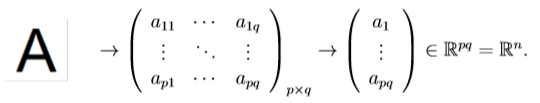
\includegraphics[width=\textwidth]{letraA_1.png}
	\end{subfigure}
	\begin{subfigure}[!h]{0.8\textwidth}
		\centering
		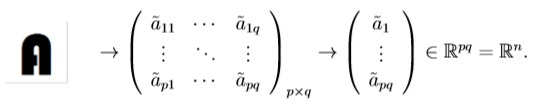
\includegraphics[width=\textwidth]{letraA_2.png}
	\end{subfigure}
	\begin{subfigure}[!h]{0.8\textwidth}
		\centering
		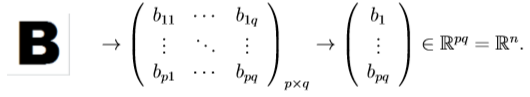
\includegraphics[width=\textwidth]{letraB.png}
	\end{subfigure}
	\caption{Classificação de caracteres. \\ Fonte: \textcite{Evelin2017}}
\end{figure}
\end{frame}


\begin{frame}{Problema de Classificação: Formulação}
\begin{block}{}
\begin{itemize}
	\item O problema de classificação trata-se de um problema de programação quadrática convexa com restrições lineares.

	\item Ele pode ser formulado como
\[
\begin{aligned}
\min_{w,b} & \quad f(w) \\
\text{s.a.} &  \quad g(w,b) \leq 0, \end{aligned}
\]
com $w\in \RR^n$ e $b\in \RR $, em que $f: \RR^{n} \rightarrow \RR$ é uma função quadrática e $g: \RR^{n+1} \rightarrow \RR^m$ é linear.
\end{itemize}
\end{block}
\end{frame}


\begin{frame}{SVM Aplicada ao Problema de Classificação}

\begin{figure}[!h] 
	\centering
	\begin{subfigure}[h]{0.3\textwidth}
		\centering
		\includegraphics[width=\textwidth]{SVM_linear}
		\caption{Linear. \label{fig1:a}}
	\end{subfigure}
	\begin{subfigure}[!h]{0.3\textwidth}
		\centering
		\includegraphics[width=\textwidth]{SVM_flexivel}
		\caption{Flexível. \label{fig1:b}}
	\end{subfigure}
	\begin{subfigure}[!h]{0.3\textwidth}
		\centering
		\includegraphics[width=\textwidth]{SVM_naolinear}
		\caption{Não Linear. \label{fig1:c}}
	\end{subfigure}
	\caption{Dados lineares, com margem flexível e não lineares. \label{fig1}\\ Fonte: \textcite{Evelin2017}}
\end{figure}
\end{frame}


\begin{frame}{Problema de Classificação: Formulação Matemática}
\begin{block}{}
Considere os conjuntos de entrada 
\[\Xset =\{x^1, \ldots , x^m \} \subset \RR^n \] 
e de treinamento 
\[\Yset=\{(x^1, y_1), \ldots , (x^m, y_m)\mid x^i \in \Xset \, e \, y_i \in \{-1,1\}\}  \subset \RR^{n+1},\]

com a partição de $\Xset$
\[ \label{conj1}
\Xset ^{+} =\{x^i \in \Xset\mid y_i=1\} \quad e \quad \Xset^{-}=\{x^i \in \Xset\mid y_i=-1\},
\]
dos conjuntos formados pelos atributos pertencentes às classes positiva e negativa, respectivamente.
\end{block}
\end{frame}


\begin{frame}

\begin{defi} 
Considere um vetor não nulo $w\in \RR^n$ e um escalar $b\in \RR$. Um \emph{hiperplano} com vetor normal $w$ e constante $b$ é um conjunto da forma $\Hset(w,b)=\{x\in \RR^n \mid w^{T}x+b=0\}$.
\end{defi}
\pause
\begin{figure}[h] 
	\centering
	\begin{subfigure}[h]{0.36\textwidth}
		\centering
		\includegraphics[width=\textwidth]{dados_treinamento}
		\caption{Dados de treinamento. \label{fig2:a}}
	\end{subfigure}
	\begin{subfigure}[h]{0.34\textwidth}
		\centering
		\includegraphics[width=\textwidth]{hiperplanos_separadores}
		\caption{Hiperplanos separadores. \label{fig2:b}}
	\end{subfigure}
	\caption{Conjunto de Dados e Hiperplanos. \label{fig2}
		\\ Fonte: \textcite{Evelin2017}}
\end{figure}
\end{frame}


\begin{frame}{Problema de Classificação: Hiperplano Ótimo}
\begin{figure}[h] 
	\centering
	\begin{subfigure}[h]{0.4\textwidth}
		\centering
		\includegraphics[width=\textwidth]{hiperplano_otimo}
		\caption{Hiperplano ótimo. \label{fig3:a}}
	\end{subfigure}
	\begin{subfigure}[h]{0.4\textwidth}
		\centering
		\includegraphics[width=\textwidth]{maxima_margem}
		\caption{Máxima margem. \label{fig3:b}}	
	\end{subfigure}
	\caption{Hiperplano Ótimo. \label{fig3}
		\\ Fonte: \textcite{Evelin2017}}
\end{figure}
\end{frame}


\begin{frame}{Problema de Classificação: Conjuntos Linearmente Separáveis}
\begin{defi} \label{def1} Os conjuntos $\Xset^{+}, \Xset^{-} \subset \RR^n$ são ditos \emph{linearmente separáveis} quando existem $w\in \RR^n$ e $b\in \RR$  tais que $w^{T}x+b>0$ para todo $x\in \Xset^{+}$ e $w^{T}x+b<0$ para todo $x\in \Xset^{-}$. O hiperplano $\Hset(w,b)$ é chamado hiperplano separador dos conjuntos $\Xset^{+}$ e $\Xset^{-}$.
\end{defi}

\begin{figure}[!h] 
	\centering
	\begin{subfigure}[h]{0.20\textwidth}
		\centering
		\includegraphics[width=\textwidth]{SVM_linear}
		\caption{Linear. \label{fig1:a}}
	\end{subfigure}
	\begin{subfigure}[!h]{0.20\textwidth}
		\centering
		\includegraphics[width=\textwidth]{SVM_flexivel}
		\caption{Flexível. \label{fig1:b}}
	\end{subfigure}
	\begin{subfigure}[!h]{0.20\textwidth}
		\centering
		\includegraphics[width=\textwidth]{SVM_naolinear}
		\caption{Não Linear. \label{fig1:c}}
	\end{subfigure}
	\caption{Dados lineares, com margem flexível e não lineares. \label{fig1}\\ Fonte: \textcite{Evelin2017}}
\end{figure}
\end{frame}


\begin{frame}{Determinação da faixa que separa os dados}
\begin{lema} \label{lema1} Suponha que os conjuntos $\Xset^{+}, \Xset^{-} \subset \RR^n$ são finitos e linearmente separáveis, com hiperplano separador $\Hset(w,b)$. Então, existem $\overline{w}\in \RR^n$ e $\overline{b}\in \RR$ tais que $\Hset(w,b)$ pode ser descrito por
\[\wbar^{T}x+\bbar =0,\]
satisfazendo
\begin{align}
\wbar^{T}x+\bbar &\geq 1, \text{ para todo } x\in \Xset^{+}, \label{eq1} \\
\wbar^{T}x+\bbar &\leq -1, \text{ para todo } x\in \Xset^{-}. \label{eq2}
\end{align}
\end{lema} 
\pause
\begin{itemize}
	\item $\Hset^{+}:=\{x\in \RR^n \mid w^{T}x+b= 1\}$ e $\Hset^{-}:=\{x\in \RR^n \mid w^{T}x+b= -1\}$ .

	\item Classificamos um novo dado $\hat{x}$ utilizando \eqref{eq1}.
\end{itemize}
\end{frame}


%\begin{frame}
%\begin{prop} \label{prop1} A projeção ortogonal de um vetor $\xbar\in \RR^n$ sobre um hiperplano afim $\Hset(w,b)$, é dada por
%	\[ \proj_{\Hset}(\xbar)= \xbar - \dfrac{w^{T}\xbar+b}{w^{T}w}w. \]
%	Além disso, a $\proj_{\Hset}(\xbar)$ satisfaz a menor distância.
%\end{prop}
%\end{frame}


\begin{frame}{Problema de Classificação: Distância entre os Hiperplanos $\Hset^{+}$ e $\Hset^{-}$}

\begin{lema}\label{lema2} A distância entre os hiperplanos $\Hset^{+}$ e $\Hset^{-}$ é dada por \[\dist(\Hset^{+} , \Hset^{-})=\dfrac{2}{\Vert w\Vert}.\]
\end{lema}

\begin{figure}[!h] 
	\centering
	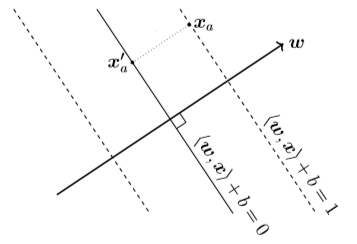
\includegraphics[width=0.40\textwidth]{distancia_hiperplanos}
	\caption{Distância entre hiperplanos. \\ Fonte: \textcite{Faisal2019}}
\end{figure}
\end{frame}


\begin{frame}{Problema de Classificação: Formulação Matemática}
\begin{block}{}
Encontrar o hiperplano ótimo implica 
\[ \max \dfrac{2}{\Vert w\Vert}  \Longleftrightarrow \min \dfrac{1}{2}\Vert w\Vert^{2}. \]
\end{block}
\pause
\begin{exampleblock}{Esboço da Demonstração}
\begin{enumerate}

	\item Seja $w^{*}:=\argmax\dfrac{2}{\Vert w\Vert}$. 

	\item Então, para todo $w\in \RR^n$,
\[ \dfrac{2}{\Vert w^{*}\Vert} \geq \dfrac{2}{\Vert w\Vert} \Rightarrow \Vert w\Vert \geq \Vert w^{*}\Vert \Rightarrow \Vert w\Vert^{2} \geq \Vert w^{*}\Vert^{2} \Rightarrow \dfrac{1}{2}\Vert w\Vert^{2} \geq \dfrac{1}{2}\Vert w^{*}\Vert^{2}. \]

	\item Portanto,
\[ \argmax\dfrac{2}{\Vert w\Vert} = \argmin\dfrac{1}{2}\Vert w\Vert^2. \]
\end{enumerate}
\end{exampleblock}
\end{frame}


\begin{frame}{Problema de Classificação: Formulação Matemática}
\begin{block}{Restrições}
Como a faixa deve separar os dados das duas classes, as seguintes restrições devem ser satisfeitas
\begin{align}
w^{T}x+b &\geq 1 , \text{ para  todo } x\in \Xset^{+}, \\
w^{T}x+b &\leq -1 , \text{ para  todo } x\in \Xset^{-}.
\end{align}

Ou de uma forma mais compacta, temos
\[ y_{i}(w^{T}x^{i}+b)\geq 1, \quad i=1, \ldots ,m. \]
\end{block}
\end{frame}


\begin{frame}{Problema de Classificação: Formulação Matemática}
\begin{block}{O Problema de Classificação pela SVM}
Portanto, o problema de encontrar o hiperplano ótimo pode ser formulado da seguinte maneira
\[ \label{eq5}
\begin{aligned}
\min_{w,b} & \quad \dfrac{1}{2} \Vert w\Vert^{2} \\
\text{s.a.} &  \quad y_i(w^{T}x^{i}+b) \geq 1, \quad i=1, \ldots , m, \end{aligned}
\]
em que $w\in \RR^{n}$ e $b\in \RR$. 
\end{block}
\end{frame}


\begin{frame}{Objetivos Gerais}
\begin{block}{}
\begin{itemize}
	\item Resumir a teoria de otimização com e sem restrições;

	\item Estudar os problemas de otimização que surgem do Aprendizado de Máquina~\cite{Ana1994,Ademir2013};

	\item Desenvolver um estudo teórico, do ponto de vista matemático, das Máquinas de Vetores Suporte~\cite{Faisal2019,Evelin2017}, em particular sua aplicação ao prolema de classificação;

	%\item Estudar a técnica de Máquinas de Vetores Suporte aplicada ao problema de classificação; 

	%\item Explorar a linguagem de programação \texttt{Julia} com a implementação de métodos de otimização;

	\item Realizar uma implementação computacional da técnica de SVM aplicada a um problema de classificação utilizando \texttt{Julia}~\cite{Bezanson:2017g}.
\end{itemize}
\end{block}
\end{frame}


%\begin{frame}{Metodologia e Resultados Esperados}
%\begin{itemize}
%	\item Estudar os aspectos teórico-matemáticos dos métodos de otimização relacionados com a Aprendizagem de Máquina, em particular relacionados à técnica de Máquinas de Vetores Suporte;
%
%	\item Realizar uma implementação computacional dos métodos de otimização e testes em bibliotecas de problemas de Aprendizagem de Máquina.
%\end{itemize}
%\end{frame}





\begin{frame}{Referências da Apresentação}
\printbibliography
\end{frame}

\begin{frame}{Agradecimento}

\begin{block}{}

\centering
\Large{\textbf{Obrigada pela atenção!}}
$$$$
{\normalsize E-mail: paulacristina\_ertel@hotmail.com }

\end{block}
\end{frame}

\end{document}